\chapter{Introduction}\label{ch:intro}

%-----------------------------------
\section{DOD / NAVY Autonomous Roadmap}
The \ac{DOD} conducted an analysis of the role of autonomy, which outlined technology gaps and predicted advancements required to meet the growing performance demands \cite{dodroadmap}.  The study amplifies the fact that autonomy is a challenging field and that it is arguably in its infancy.  The roadmap attempts to guide decision makers in ensuring capitalization of under-utilized technology and succinct awareness of technical challenges limiting the current state of the art.  Figure~\ref{fig:dod_roadmap} outlines these elements at increasing scope of control comprised of various technology portfolios.  
\begin{figure}[h!]
 \centering
  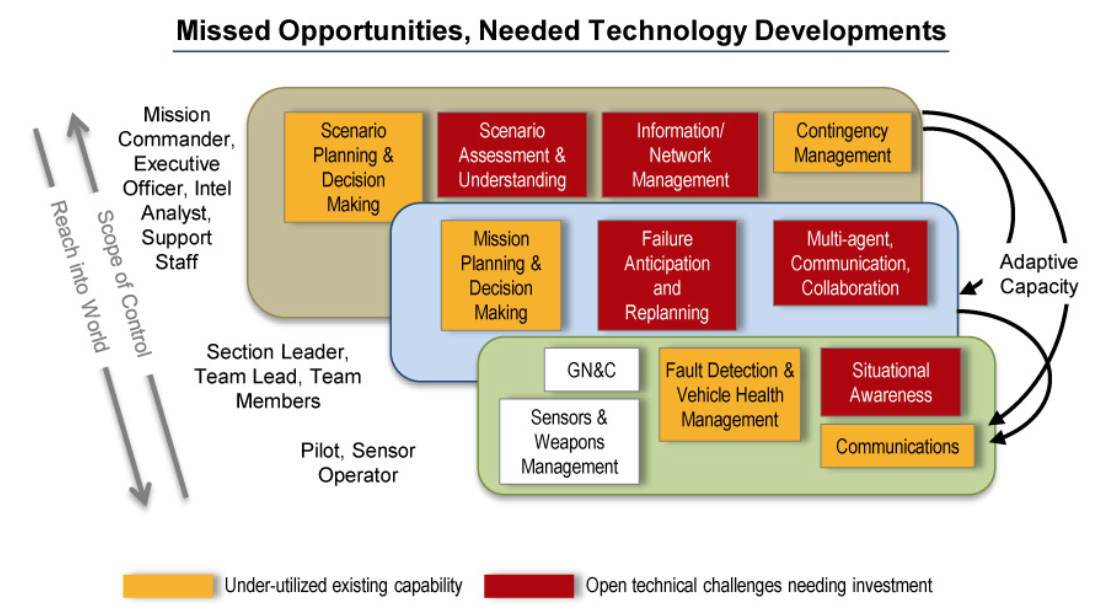
\includegraphics[width=1.0\textwidth]{DOD_roadmap.png}
  \caption{DOD Autonomy Roadmap.  Source \cite{dodroadmap}.}
  \label{fig:dod_roadmap}
\end{figure}
The language referenced in the roadmap often recommends that machine learning and/or artificial intelligence is needed for elements such as \enquote{Fault Detection.}  On the lowest level, the roadmap annotates the use of \ac{GNC} as neither needing improvement or current technology being underutilized.  An in-depth look at the current state of the art with respect to \ac{GNC} reveals that \ac{GNC} is still very costly and arguably antiquated.  Research of adaptive control as applied to \ac{GNC} offers new strategies offering improved performance and future reduced cost.

%-----------------------------------
\section{Challenges in Designing Versatile Controllers}
The \ac{UAS} has evolved tremendously over the past decade.  Miniature autopilots have gotten smaller and cheaper with more sensitive and redundant sensor packages largely due to the cellular phone industry accelerating \ac{MEMS} technology.  The ability to manufacture these autonomous systems at fractions of the cost enables the advancement in multiple cooperative \ac{UAS} applications including swarming capability.  This ability to mass-produce large quantities of \ac{UAS}'s poses an interesting challenge.  Even though the price has gone down and the performance has gone up, there still exists a significant amount of man-hours dedicated to sensor calibration and autopilot control law configuration and tuning for optimal performance.  

Over the past decade \ac{UAS} avionics have drastically improved, but the fundamental control law algorithms have not changed.  The \ac{PID} architecture found its origin in automatic ship steering applications in 1922 \cite{minorsky1922pid}.  Conventional control law architectures for \ac{UAS}s predominately still use \ac{PID} controllers.  Their architecture offers a well understood and predictable behavior for the class of linear systems.  For this reason, it is well suited for the aviation application.  The detriment of \ac{PID} control is that its application is mostly constrained by its use on a linear plant and most aerospace applications are non-linear and time varying.   An aircraft's control authority that increases proportionally to dynamic pressure is one example of significant changes in aerodynamic non-linear control behavior.  In this case, the \ac{PID} controller's robustness to changes in velocity and/or density altitude is not guaranteed and for most aircraft has to be delicately handled with lookup tables produced from hours of flight test for given configurations.

Conventional controllers (\ac{PID}) are difficult to tune and achieving an adequately tuned controller requires a significant amount of time and resources.  These difficulties can arise because of many uncertainties with respect to the aircraft as outlined in the following three subsections.

\subsection{Unknown Constant Airframe Parameters}
In the case where airframes are assembled by the same manufacturer, all aircraft still require a tedious quality assurance check.  Physical aspects of the airframes such as \ac{CG}, control surface deflection/calibration/speed, and airframe alignment all can drastically vary within the same delivered batch of airframes.  Additionally, these miniature \ac{UAS}s experience hard landings, crashes, and/or damage in transportation, which all can affect aerodynamic handling qualities.

\subsection{Unknown Non-Constant Airframe Parameters}
Aircraft with large airspeed envelopes or various configurations (\ac{VTOL}, flaps, retractable landing gear), exhibit changing dynamics that challenge conventional \ac{PID} robustness.  Because these dynamics are changing drastically, the \ac{PID} controllers either underperform or have to be over designed with ad-hoc gain scheduling techniques which significantly increases the controller's already complex tuning process.  

\subsection{Fault Tolerance}
If an aircraft exhibits airframe faults or battle damage, the desirable outcome results in the controller achieving robust performance.  Classical \ac{PID} controllers have limited to no ability to cope with these types of failures.  Conventional methods require a priori knowledge of the failure scenario. Reconfiguration schemes are developed for specific failures, further complicating designs.

%-----------------------------------
\section{Problem Formulation and Thesis Organization}

This thesis addresses a problem of shortening the time for developing and fielding a new autonomous aerial vehicle by utilizing an adaptive controller, which relaxes some of the traditional constraints and assures better robustness in the case of airframe configuration variation, various uncertainties, and faults.  

To address the formulated problem, this thesis is organized as follows.

Chapter~\ref{ch:overview} provides an overview of modern adaptive control.  The brief history of adaptive control is introduced to further amplify the specific use case for aerospace applications.  The adaptive control architecture is compared with conventional feedback controllers (\ac{PID}) to clarify the distinction between the two approaches for stable and robust control.  The \ac{MRAC} architecture is defined in order to articulate the difference between the \ac{MRAC} architecture and the specific modifications utilized in this research to formulate the \Lone adaptive controller.

Chapter~\ref{ch:adaptive_controller} outlines the proposed adaptive controller architecture used instead of conventional less-robust controllers.  It addresses why the architecture must take the form of indirect adaptive control vice direct adaptive control.  The definition of estimated parameters are defined with respect to the aerodynamics model derived in Appendix~\ref{appendix:dynamics_model}.  The filter section of the controller used to bandwidth limit the controller is defined with respect to the specific three parameter model chosen for this research.  The \Lone adaptive controller discretization process is reviewed with respect to methods implemented to achieve integration on a \ac{COTS} autopilot, which is described in Chapter~\ref{ch:platform}.

Chapter~\ref{ch:platform} discusses the \ac{COTS} autopilot and flight stack code chosen for this research.  It also covers the \ac{GCS} and \ac{SITL} infrastructure which was heavily utilized for initial code development, testing, and validation.  Chapter~\ref{ch:platform} follows with the major steps undertake to prototype two airframes to be used in the flight testing of the proposed controller.

Chapter~\ref{ch:performance} and \ref{ch:recomendations} describe the results of computer simulations and flight tests, respectively.  Chapter~\ref{ch:recomendations} also outlines the shortcomings of the \ac{COTS} autopilot architecture and improvements specific to the \Lone adaptive controller.

The thesis concludes with Chapter~\ref{ch:conclusion} providing conclusions.






